\documentclass[eng,printmode,oneside]{mgr}
\usepackage[MeX]{polski}
\usepackage[utf8]{inputenc}
\usepackage[T1]{fontenc} 
\usepackage{graphicx}
\usepackage{subfigure}
\usepackage{psfrag}
\usepackage{amsmath}
\usepackage{amsfonts}
%\usepackage{supertabular}
\usepackage{array}
\usepackage{tabularx}
\usepackage{hhline}
\usepackage{rev}
%\usepackage{framed}
\usepackage{color}
\usepackage{url}
%\usepackage[notref]{showkeys}
%\usepackage{showlabels}
\usepackage{float}
%\usepackage{tikz}
\usepackage{enumitem} 
\usepackage{graphicx}       
\usepackage{rotating}       % pakiet umożliwiający obracanie rysunków
\usepackage{subfigure}      % pakiet umożliwiający tworzenie podrysunków
\usepackage{epic}           
\usepackage{listings}       % pakiet dedykowany zrodlom programow
\usepackage{verbatim}       % pakiet dedykowany rozmaitym wydrukom tekstowym
\usepackage{amssymb}        % pakiet z rozmaitymi symbolami matematycznymi
\usepackage{amsmath}        % pakiet z rozmaitymi środowiskami matematycznymi
\usepackage[polish]{babel}  % pakiet lokalizujący dokument w języku polskim
\usepackage[OT4]{fontenc}
\usepackage[utf8]{inputenc}
\usepackage{bm}
\usepackage{gensymb}
\usepackage{booktabs}
\usepackage{epstopdf}
\usepackage{amssymb}
\usepackage[utf8]{inputenc}
\usepackage{amsmath}
\usepackage{amsfonts}
\usepackage{amssymb}
\usepackage{graphics}
\usepackage[]{algorithmic} %pseudocode
\usepackage[]{algorithm2e} %pseudocode
\usepackage{float}
\usepackage{csquotes}
\usepackage{epsfig}
%\usepackage{hyperref}
\usepackage{wrapfig} 
\reviewer{dypl}{0.2}{0.2}{0.67}
\reviewer{prof}{0.2}{0.6}{0.2}
\def\bp{\begin{review}[prof]}
\def\ep{\end{review}}
\def\bdypl{\begin{review}[dypl]}
\def\edypl{\end{review}}
\newcommand{\R}{I\!\!R} 
\newtheorem{theorem}{Twierdzenie}[section] 
\newcommand\numberthis{\addtocounter{equation}{1}\tag{\theequation}}
\newenvironment{myitemize}%
 { \begin{list}{\labelitemi}%
   {
      \setlength{\itemsep}{0mm}%
      \setlength{\topsep}{6pt}%
      \setlength{\leftmargin}{5mm}%
     \setlength{\parsep}{1mm}%
    }
  }
{\end{list}
}
\newcounter{mycount}
\newenvironment{MYenumerate}%
 {\begin{list}{\arabic{mycount}.}%
   {\usecounter{mycount}%
%      \setlength{\topsep}{12pt}%
      \setlength{\topsep}{6pt}%
      \setlength{\itemsep}{0mm}%
      \setlength{\leftmargin}{7mm}%
     \setlength{\parsep}{1mm}%
    }%
 }%
{\end{list}}
\newenvironment{todo}
{
\label{todo}
\color{red} [
}
{]
}
%%%%%%%%%chapter no new page%
\usepackage{etoolbox}

\makeatletter
\patchcmd{\chapter}{\if@openright\cleardoublepage\else\clearpage\fi}{}{}{}
\makeatother
%%%%%%%%%%%%%
\title{?}
\engtitle{?}

\author{inż. Bernard Malec}
\supervisor{Prof.\ dr hab.\ inż.\ Alicja Mazur}


\field{Automatyka i Robotyka (AIR)}
\specialisation{Robotyka (ARR)}

%\includeonly{mch0,mch1,mch2,mch3,mch4,bibl}
%\includeonly{mch3}

\begin{document}
\bibliographystyle{plabbrv} %BibTeX polski styl bibliografii 

% te ozdobniki dodaje się dopiero na końcu 
%\maketitle

\chapter{Model satelity typu free-floating}
\section{Model we współrzędnych uogólnionych}
Robot free-floating z manipulatorem to nienapędzana platforma(baza) z zamontowanym na niej napędzanym manipulatorem. Robot taki znajdująca się w przestrzeni kosmicznej w stanie mikrograwitacji(nieważkości).
\par W szczególności w rozważanym robocie platformą będzie jednolita prostokątna płyta, a za manipulator posłuży manipulator RR.
\par Rozważanego robota free-floating z manipulatorem przedstawiono na rys 1. \par Robot taki jest przyjemny ze względów praktycznych. Do badań eksperymentalnych bowiem, można wykorzystać płaską granitową płytę, po której baza może ślizgać się bez tarcia. %, a siły grawitacji nie mają wpływu na dynamikę.
Dzięki temu testy można przeprowadzać na ziemi, a nie w warunkach mikrograwitacji.

\par Do wyprowadzenia modelu we współrzędnych uogólnionych weźmy następujące współrzędne
\begin{equation}
q=\left(
\begin{array}{c}
q_b\\
q_r\\
\end{array}
\right),
\end{equation}
gdzie $q_b=(x,y,\theta)^T$ - wektor współrzędnych uogólnionych bazy, $q_r=(q_1,q_2)^T$ - wektor współrzędnych przegubowych manipulatora. 
\par Równania dynamiki we współrzędnych uogólnionych takiego robota można, ponownie korzystając z formalizmu Langrange'a, zapisać jako\\
\begin{equation}
\label{wrsdad}
H(q)\ddot{q}+C(q,\dot{q})\dot{q}=
\left(
\begin{array}{c}
0\\
u\\
\end{array}
\right).
\end{equation}\\
Brak wektora sił potencjalncyh $D(q)$ wynika z braku grawitacji. \par Sterowanie $u$ pojawia się tylko w dolnej części równania dynamiki (\ref{wrsdad}), ponieważ dotyczy jedynie manipulatora, jako że baza jest nienapędzana.
%H\ddot{q}+c=
%\begin{bmatrix}
%    H_b  &H_{bm}\\
%    H_{bm}^T  &H_m \\
%\end{bmatrix}
%\left(
%\begin{array}{c}
%\ddot{q_b}\\
%\ddot{q_m}\\
%\end{array}
%\right)
%+
%\left(
%\begin{array}{c}
%c_b\\
%c_m\\
%\end{array}
%\right)
%=
%\left(
%\begin{array}{c}
%0\\
%u\\
%\end{array}
%\right).
%\end{equation}\\
\section{Model we współrzędnych barycentrycznych}
Jeśli środek masy robota free-floating z manipulatorem ma pozostać nieruchomy podczas działania algorytmu, konieczne jest zamodelowanie dynamiki we współrzędnych barycentrycznych.\\
\par Położenie środka masy robota free-floating z manipulatorem można wyliczyć z definicji jako
\begin{equation}
\left(\sum\limits^w_{i=1}m_i\right)\phi_b=\sum\limits^w_{i=1}m_ir_i,
\end{equation}
gdzie $r_i$ to środek masy członu $i$ robota w podstawowym układzie współrzędnych, a  $m_i$ to masa członu $i$. $w$ to liczba członów robota. W naszym przypadku $w$ wynosi trzy, robot posiada bowiem jedną bazę i dwa ramiona.\\
$\phi_b$ to współrzędne barycentryczne układu, czyli
\begin{equation}
\label{baro}
\phi_b=
\left(
\begin{array}{c}
\bar{x}\\
\bar{y}\\
\theta\\
\end{array}
\right)=
\frac{\sum\limits^w_{i=1}m_ir_i}{\sum\limits^w_{i=1}m_i}.
\end{equation}
całkowite współrzędne barycentryczne $\phi$ mają postać
\begin{equation}
\phi=
\left(
\begin{array}{c}
\phi_b\\
q_r\\
\end{array}
\right).
\end{equation}
Model we współrzędnych barycentrycznych można wyrazić jako
\begin{equation}
\bar{H}\ddot{\phi}+\bar{C}\dot{\phi}
=
\left(
\begin{array}{c}
0\\
u\\
\end{array}
\right),
\end{equation}
%\bar{H}\ddot{\phi}+\bar{c}
%=
%\begin{bmatrix}
%    \bar{H}_b  &\bar{H}_{bm}\\
%    \bar{H}_{bm}^T  &\bar{H}_m \\
%\end{bmatrix}
%\left(
%\begin{array}{c}
%\ddot{\phi_b}\\
%\ddot{q_m}\\
%\end{array}
%\right)
%+
%\left(
%\begin{array}{c}
%\bar{c}_b\\
%\bar{c}_m\\
%\end{array}
%\right)
%=
%\left(
%\begin{array}{c}
%0\\
%u\\
%\end{array}
%\right),
%\end{equation}

Macierze $\bar{H}$ i $\bar{C}$ uzyskuje się przez przeliczenie energii kinetycznej do układu współrzędnych barycentrycznych i wykorzystanie formalizmu Lagrang'e dla nowej energii kinetycznej.\\

\chapter{Odsprzęganie wejściowo-wyjściowe dla robota free-floating z manipulatorem}

Ponieważ baza robota free-floating z manipulatorem nie jest napędzana, do odsprzęgania wejściowo-wyjściowego nie można zastosować podstawowego algorytmu Yamamoto i Yun'a. Do realizacji zadania śledzenia trajektorii w przestrzeni zadaniowej wykorzystamy więc algorytm z rozszerzonymi funkcjami wyjściowymi.
\par Algorytm ten stosować można zarówno dla modelu robota free-floating z manipulatorem we współrzędnych uogólnionych jak i we współrzędnych barycentrycznych. Wybór modelu należy podporządkować rodzajowi zadania jakie ma zostać wykonane. Jeśli środek masy ma pozostać nieruchomy wykorzystać należy model we współrzędnych barycentrycznych, natomiast gdy środek masy ma się przemieszczać należy użyć modelu we współrzędnych uogólnionych.
\par Przy wyprowadzaniu algorytmu wykorzystamy model dynamiki we współrzędnych uogólnionych. Algorytmu dla modelu we współrzędnych barycentrycznych wyprowadza się analogicznie, podstawiając jedynie za współrzędne uogólnione $q$ i macierze  $H$ i $C$ ich odpowiedniki w modelu we współrzędnych barycentrycznych, tj.  współrzędne barycentryczne $\phi$ i macierze $\bar{H}$ i $\bar{C}$.

\par Korzystamy z algorytmu z rozszerzonymi funckjami wyjściowymi, więc postać funkcji wyjściowej będzie zależeć więc od całej konfiguracji $q$.
\begin{equation}
y=k(q)
\end{equation}
\section{Algorytm}
Przy wyprowadzaniu algorytmów odsprzęgania wejściowo-wyjściowego dla manipulatora mobilnego linearyzowaliśmy jego dynamikę w celu ułatwienia obliczeń. W przypadku robota free-floating z manipulatorem linearyzacja taka jest kłopotliwa, ponieważ tylko manipulator jest napędzany. Aby nie utrudniać sobie zadania i pokazać, że linearyzacja dynamiki nie jest konieczna, nie zastosujemy jej przy wyprowadzaniu algorytmu odsprzęgania wejściowo-wyjściowego dla robota free-floating z manipulatorem.
\par Struktura algorytmu nie zmienia się i nadal składa się z dwóch pętli sprzężenia zwrotnego: pierwsza przekształca układ do postaci liniowej typu "podwójny integrator", druga steruje uzyskanym układem liniowym.
\par Prawo sterowania pierwszej pętli wyprowadza się analogicznie jak w przypadku manipulatorów mobilnych.
\par Zróżniczkujmy wszystkie elementy wektora $y(q)$ dwukrotnie po czasie
\begin{equation}
\dot{y}_i=\dfrac{\partial k_i(q)}{\partial q}\dot{q}=J_i\dot{q},
\end{equation}
\begin{equation}
\ddot{y}_i=\dot{q}^T\dfrac{\partial^2k_i(q)}{\partial q^2}\dot{q}+J_i\ddot{q}=P_i+J_i\ddot{q},
\end{equation}
gdzie
\begin{equation}
J_i=\dfrac{\partial k_i(q)}{\partial q},
\end{equation}
\begin{equation}
P_i=\dot{q}^T\dfrac{\partial^2k_i(q)}{\partial q^2}\dot{q}.
\end{equation}
Zapiszmy $\dot{y}$ i $\ddot{y}$ w postaci wektorowej
\begin{equation}
\dot{y}=J\dot{q},
\end{equation}
\begin{equation}
\label{ypplol}
\ddot{y}=P+J\ddot{q},
\end{equation}
gdzie
\begin{equation}
P=
\left(
\begin{array}{c}
P_1\\
P_2\\
\vdots\\
P_m\\
\end{array}
\right),
\end{equation}
\begin{equation}
J=
\left(
\begin{array}{c}
J_1\\
J_2\\
\vdots\\
J_m\\
\end{array}
\right),
\end{equation}
$m$ jest liczbą sterowań, $m=\dim(u)=\dim(q_r)$.
\par Korzystając z dynamiki we współrzędnych uogólnionych (\ref{wrsdad}) zapiszmy $\ddot{q}$  jako
\begin{equation}
\label{qpplol}
\ddot{q}=H^{-1}
\left[
\left(
\begin{array}{c}
0\\
u\\
\end{array}
\right)
-C\dot{q}
\right].
\end{equation}
Podstawmy teraz  (\ref{qpplol}) do (\ref{ypplol})
\begin{equation}
\ddot{y}=P+J
H^{-1}
\left[
\left(
\begin{array}{c}
0\\
u\\
\end{array}
\right)
-C\dot{q}
\right],
\end{equation}
więc
\begin{equation}
\ddot{y}=
P-JH^{-1}C\dot{q}
+
JH^{-1}\left(
\begin{array}{c}
0\\
u\\
\end{array}
\right).
\end{equation}
Zapiszmy więc $\ddot{y}$ następująco
\begin{equation}
\ddot{y}=
F+G\left(\begin{array}{c}
0\\
u\\
\end{array}
\right),
\end{equation}
gdzie
\begin{equation}
F=P-JH^{-1}C\dot{q},
\end{equation}
\begin{equation}
G=JH^{-1}.
\end{equation}
macierz $G$ zapiszmy jako $G=[G_1|G_2]$. Macierz $G_2$ jest rozmiaru $m\times m$.\\
Wektor $\ddot{y}$ można zapisać wtedy jako
\begin{equation}
\label{helloasdasda}
\ddot{y}=F+G_2u.
\end{equation}
Prawo sterowania pętli linearyzującej jest więc następujące
\begin{equation}
\label{ulol}
u=G_2^{-1}(-F+\zeta).
\end{equation}
Po wykorzystaniu sterowania (\ref{ulol}) w (\ref{helloasdasda}) otrzymamy układ liniowy
\begin{equation}
\label{helloasdasdaasdasdasd}
\ddot{y}=\zeta.
\end{equation}
Za wysterowanie liniowym układem (\ref{helloasdasdaasdasdasd}) odpowiada druga pętla. Zrealizować ją, można jako regulator PD z korekcją (\ref{PD}).

\subsection{Badania symulacyjne}
Podrozdział ten poświęcony jest symulacji algorytmu odsprzęgania wejściowo-wyjściowego dla robota free-floating z manipulatorem.\\
\par Algorytm zbadano na obu przedstawionych w pracy modelach dynamiki. W badaniach użyto identyczne konfiguracje początkowe $q_b(0),q_r(0)$ i tą samą trajektorię zadaną $y_d(t)$ , w celu porównania obu modeli.\\
Parametry geometryczne i masowe ustalono jako: $l_1$=1m, $l_2$=1m, $m_0=$20kg, $m_1$=$m_2$=10kg.\\
Początkowa konfiguracja bazy $q_b(0)$ we współrzędnych uogólnionych była równa
\begin{center}
$q_b(0)=
\left(
\begin{array}{c}
   x(0) \\
    y(0) \\
    \theta(0)\\
\end{array}
\right)=
\left(
\begin{array}{c}
    ? \\
     ? \\
\end{array}
\right).$
\end{center}
We współrzędnych barycentrycznych konfigurację bazy $\phi_b(0)$ możemy zapisać jako
\begin{center}
$\phi_b(0)=
\left(
\begin{array}{c}
   \bar{x}(0) \\
   \bar{y}(0) \\
    \theta(0)\\
\end{array}
\right)=
\left(
\begin{array}{c}
    ? \\
     ? \\
\end{array}
\right),$
\end{center}
co wynika to z przekształcenia (\ref{baro}). W naszym wypadku $\bar{x}$ i $\bar{y}$ będą równe
\begin{center}$
\begin{array}{c}
\bar{x}= \dfrac{{m_2} \left({l_1}
   c_{01}+\dfrac{1}{2} {l_2} c_{012}\right)}{{m_1}+{m_2}+{m_0}}+\dfrac{{l_1} {m_1} c_{01}}{2   ({m_1}+{m_2}+{m_0})}+x,\\
   \bar{y}= \dfrac{{m_2} \left({l_1} s_{01}+\dfrac{1}{2} {l_2} s_{012}\right)}{{m_1}+{m_2}+{m_0}}+\dfrac{{l_1} {m_1} s_{01}}{2
   ({m_1}+{m_2}+{m_0})}+y.
   \end{array}
$\end{center}
Początkowa konfiguracja manipulatora była równa 
\begin{center}
$q_r(0)=
\left(
\begin{array}{c}
   q_1(0) \\
    q_2(0) \\
\end{array}
\right)=
\left(
\begin{array}{c}
    ? \\
     ? \\
\end{array}
\right).$
\end{center}
Prędkości początkowe $\dot{q}(0)$ były równe zeru.  \\
Podczas badań odsprzęgnięto współrzędne $x$ i $y$ efektora w podstawowym układzie odniesienia ($X_0$,$Y_0$).\\
Funkcja wyjścia we współrzędnych uogólnionych $y(q_b,q_r)$ ma postać\\
\begin{center}
$y(q_b,q_r)=
\left(
\begin{array}{c}
    x + l_1c_{01} + l_2c_{012}\\
    y + l_1s_{01} + l_2s_{012}\\
\end{array}
\right).$
\end{center}
Po przekształceniu $q_b$ do $\phi_b$ otrzymamy funkcję wyjścia we współrzędnych barycentrycznych
\begin{center}
$y(\phi_b,q_r)=
\left(
\begin{array}{c}
   \dfrac{{l_1} ({m_1}+2  {m_0}) c_{01}+ {l_2} (2
    {m_1}+ {m_2}+2  {m_0}) c_{012}+2  \bar{x}
   ( {m_1}+ {m_2}+ {m_0})}{2( {m_1}+ {m_2}+ {m_0})}\\
   \dfrac{ {l_1}   ( {m_1}+2  {m_0}) s_{01}+ {l_2} (2  {m_1}+ {m_2}+2
    {m_0}) s_{012}+2    \bar{y} ( {m_1}+ {m_2}+ {m_0})}{2
   ( {m_1}+ {m_2}+ {m_0})}
\end{array}
\right).$
\end{center}
Funkcje wyjścia miały następujące wartości początkowe 
\begin{center}
$y(q_b(0),q_r(0))=
\left(
\begin{array}{c}
    ? \\
     ? \\
\end{array}
\right).$
\end{center}
\begin{center}
$y(\phi_b(0),q_r(0))=
\left(
\begin{array}{c}
    ? \\
     ? \\
\end{array}
\right).$
\end{center}
Wektor pochodnych $\dot{y}$ był zerowy.\\

Wybrano następujące trajektorie zadane $y_d(t)$ 
\begin{center}
$y_d(t)=
\left(
\begin{array}{c}
    ?\\
    ?\\
\end{array}
\right).$
\end{center}
Błąd początkowy $e(t)=y_d(t)-y(t)$ i jego pochodna były równe
\begin{center}
$e(0)=
\left(
\begin{array}{c}
   ?\\
    ?\\
   \end{array}
\right), \hspace{1.5cm}
\dot{e}(0)=
\left(
\begin{array}{c}
    ?\\
    ?\\
\end{array}
\right).$
\end{center}
Do sterowania układem liniowym użyto regulator PD z korektą (\ref{PD}) z nastawami $K_d=4$, $K_p=2$.
W badaniach wykorzystano środowisko Matlab/Simulink. \\
Rezultaty badań przedstawiono poniżej.
\subsection{Wyniki dla modelu we współrzędnych uogólnionych}
Sterować można tylko dwoma przegubami manipulatora, a więc odsprząc dwie współrzędne efektora.\\


\begin{figure}[H]
\centering
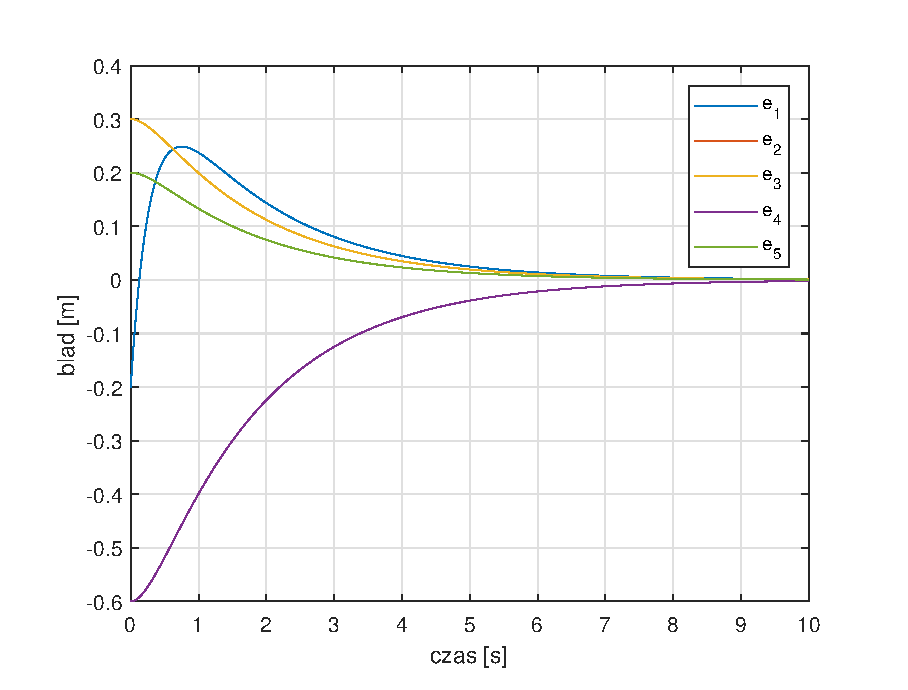
\includegraphics[width=.6\linewidth]{pics/ZRe}
\caption{Przebieg błędu}
\label{fig:regnad}
\end{figure}

\begin{figure}[H]
\centering 
\begin{minipage}{.5\textwidth}
  	\centering
  	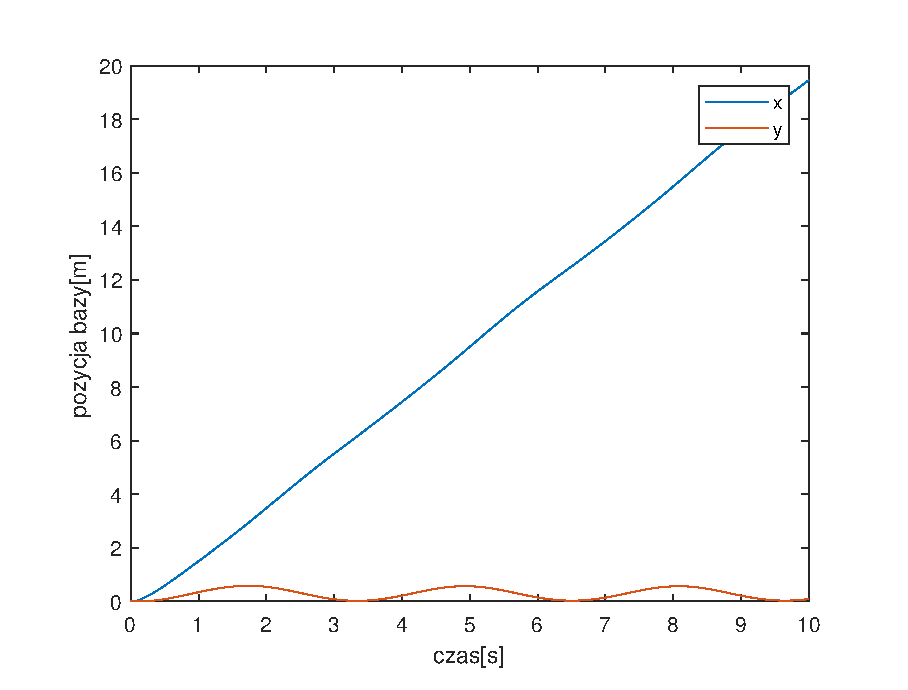
\includegraphics[width=.99\linewidth]{pics/ZRx}
  	
  	\label{fig:sub1}
\end{minipage}%
\begin{minipage}{.5\textwidth}
 	\centering
    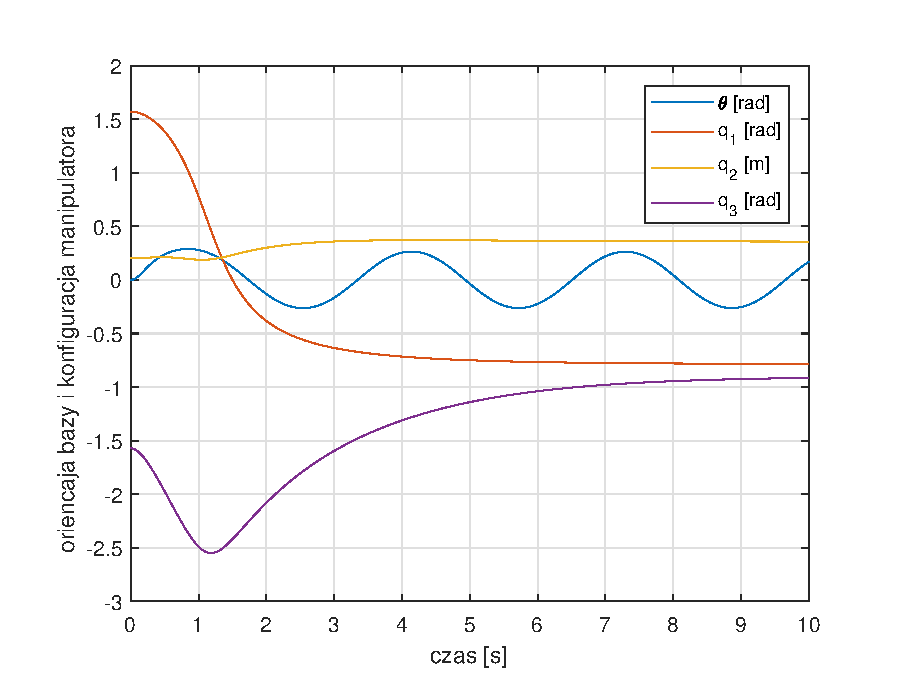
\includegraphics[width=.99\linewidth]{pics/ZRq}
 	
  	\label{fig:sub1}
\end{minipage}%
\caption{Przebieg konfiguracji bazy i manipulatora}
\label{fig:regnad}
\end{figure}


\end{document}
